\documentclass[12pt]{article}

\usepackage[utf8]{inputenc}
\usepackage{amsmath}
\usepackage{graphicx}
\usepackage[margin=1in]{geometry}
\usepackage{hyperref}
\usepackage{caption}
\captionsetup{justification=centering}

\title{\Huge\centering Biomaterials Notes}
\author{Taught by Adam Celiz \\ Notes by Harsh Agrawal}
\date{\today}

\begin{document}

\maketitle
\tableofcontents
\newpage

\section{Introduction}
\subsection{Need for Biomaterials}
Biomaterials have been used in different capacities for more than a thousand
years. Most early biomaterials were metals such as gold braces in ancient Egypt
(1500 B.C.). Metals were usually used as they didn't degrade.

On the basis of biological integration, biomaterials can be classified into:
\begin{itemize}
    \item Implants
    \item Transplants
    \item Prostheses
\end{itemize}

An \textbf{implant} is an object that is inserted or embedded surgically into
the body. This includes leg implants, breast implants, dental implants, etc.
Some common issues with implants include:
\begin{itemize}
    \item \textbf{Problem 1}: No manmade material available today can completely match the biomechanical characteristics of living tissues and thus true integration is often unattainable.
    \item \textbf{Problem 2}: No manmade material can self repair.
    \item \textbf{Problem 3}: No manmade material is capable of adjusting its
          structure and properties to changes in the environment or to mechanical
          that it encounters.
\end{itemize}

An \textbf{transplant} is typically a tissue or organ that is moved from one
body or body part to another. This includes heart transplants, skin grafts,
etc. On the basis of the origin of tissue / organ, transplants can be
categorized into:
\begin{itemize}
    \item \textbf{Autografts}: Transplants from another site of the patient's body. It is often the most desirable option as it reduces the chance of infection and immune-rejection. However, it is often detrimental to the donor site. Some examples include skin grafts, bone grafts, etc.
    \item \textbf{Allografts}: Transplant from another human. This is often less desirable than autografts due to the chances of immune rejection. There is also a risk of disease transmission. An example is kidney transplants.
    \item \textbf{Xenografts}: Transplant from another species. This is often the least desirable option as there is a high risk of immune rejection and disease transmission. We still do not fully understand the long-term effects of xenografts. An example is heart valves taken from pigs during valve replacement surgeries.
\end{itemize}

A \textbf{prosthesis} is an artificial device used inside the body to replace
or augment a diseased / damaged part. An example is the full hip replacement
prosthesis.
\subsection{Pre-requisite Cell Biology}
\subsubsection{Cell Membrane}
The cell membrane is composed of a phospholipid bilayer with embedded proteins
bound to sugar and cholesterols. Key properties of the cell membrane include:
\sloppy
\begin{itemize}
    \item \textbf{Isolation}: The cell membrane insulates and isolates the cell from the external environment.
    \item \textbf{Selective permeability}: The cell membrane allows certain substances to pass through while blocking others. It allows for the free diffusion of hydrophobic non-polar and small polar molecules. It also facilitates protein-mediated transport of large polar molecules and ions.
    \item \textbf{Controls Trafficking}: The cell membrane controls the movement of substances into and out of the cell.
    \item \textbf{Key Role in Signalling}: The cell membrane plays a key role in signalling and signal recognition.
    \item \textbf{Phagocytotic Function}: The cell membrane allows for endocytosis of fluids and large particles.
\end{itemize}

\begin{figure}[h]
    \centering
    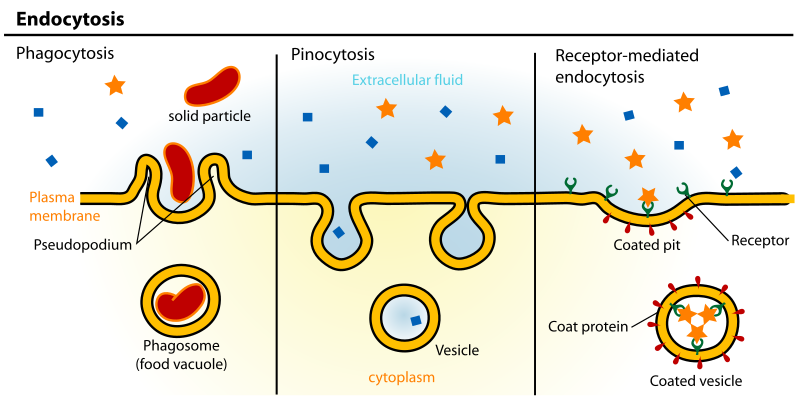
\includegraphics[width=1\textwidth]{figures/section_2/endocytosis.png}
    \caption{Figure shows the different types of endocytosis}\label{fig:endocytosis}
\end{figure}

\textbf{Endocytosis} is a cellular process in which substances are brought into the cell. The material to be internalized is surrounded by an area of cell membrane, which then buds off inside the cell to form a vesicle containing the ingested materials.\footnote{Source: \url{https://en.wikipedia.org/wiki/Endocytosis}} There are four primary pathways of endocytosis:
\begin{itemize}
    \item \textbf{Clathryn-Mediated Endocytosis}: mediated by the production of small (approx. 100 nm in diameter) vesicles that have a morphologically characteristic coat made up of the cytosolic protein \textbf{clathrin}. It is also called receptor-mediated endocytosis.
    \item \textbf{Caveolae-Mediated Endocytosis}: mediated by non-clathryn coated membrane buds made up of cholesterol-binding proteins called caveolins. The name comes from `caveolae' which are small (approx. 50 nm in diameter) flask-shape pits in the membrane that resemble the shape of a cave.
    \item \textbf{Pinocytosis}: Non-specific uptake of extra-cellular fluid into the cell through small vescicles called pinosomes.
    \item \textbf{Phagocytosis}: cells, primarily some immune cells such as macrophages, engulf solid particles like bacteria, debris, and dead cells using large vescicles called phagosomes, which fuse with lysosomes for digestion.
\end{itemize}

\textbf{Exocytosis} is the process of emptying membrane-bound vesicles into the extra-cellular region. This is used to release hormones, neurotransmitters, and other signaling molecules. It is also used to insert cell-surface proteins into the cell membrane.

\textbf{Lysosomes} are membrane-bound vesicles filled with hydrolytic enzymes (very low pH) capable of digesting a variety of macromolecules. These are also called `suicidal bags'.

\subsubsection{Cytoskeleton and Motor Proteins}
\begin{figure}[h]
    \centering
    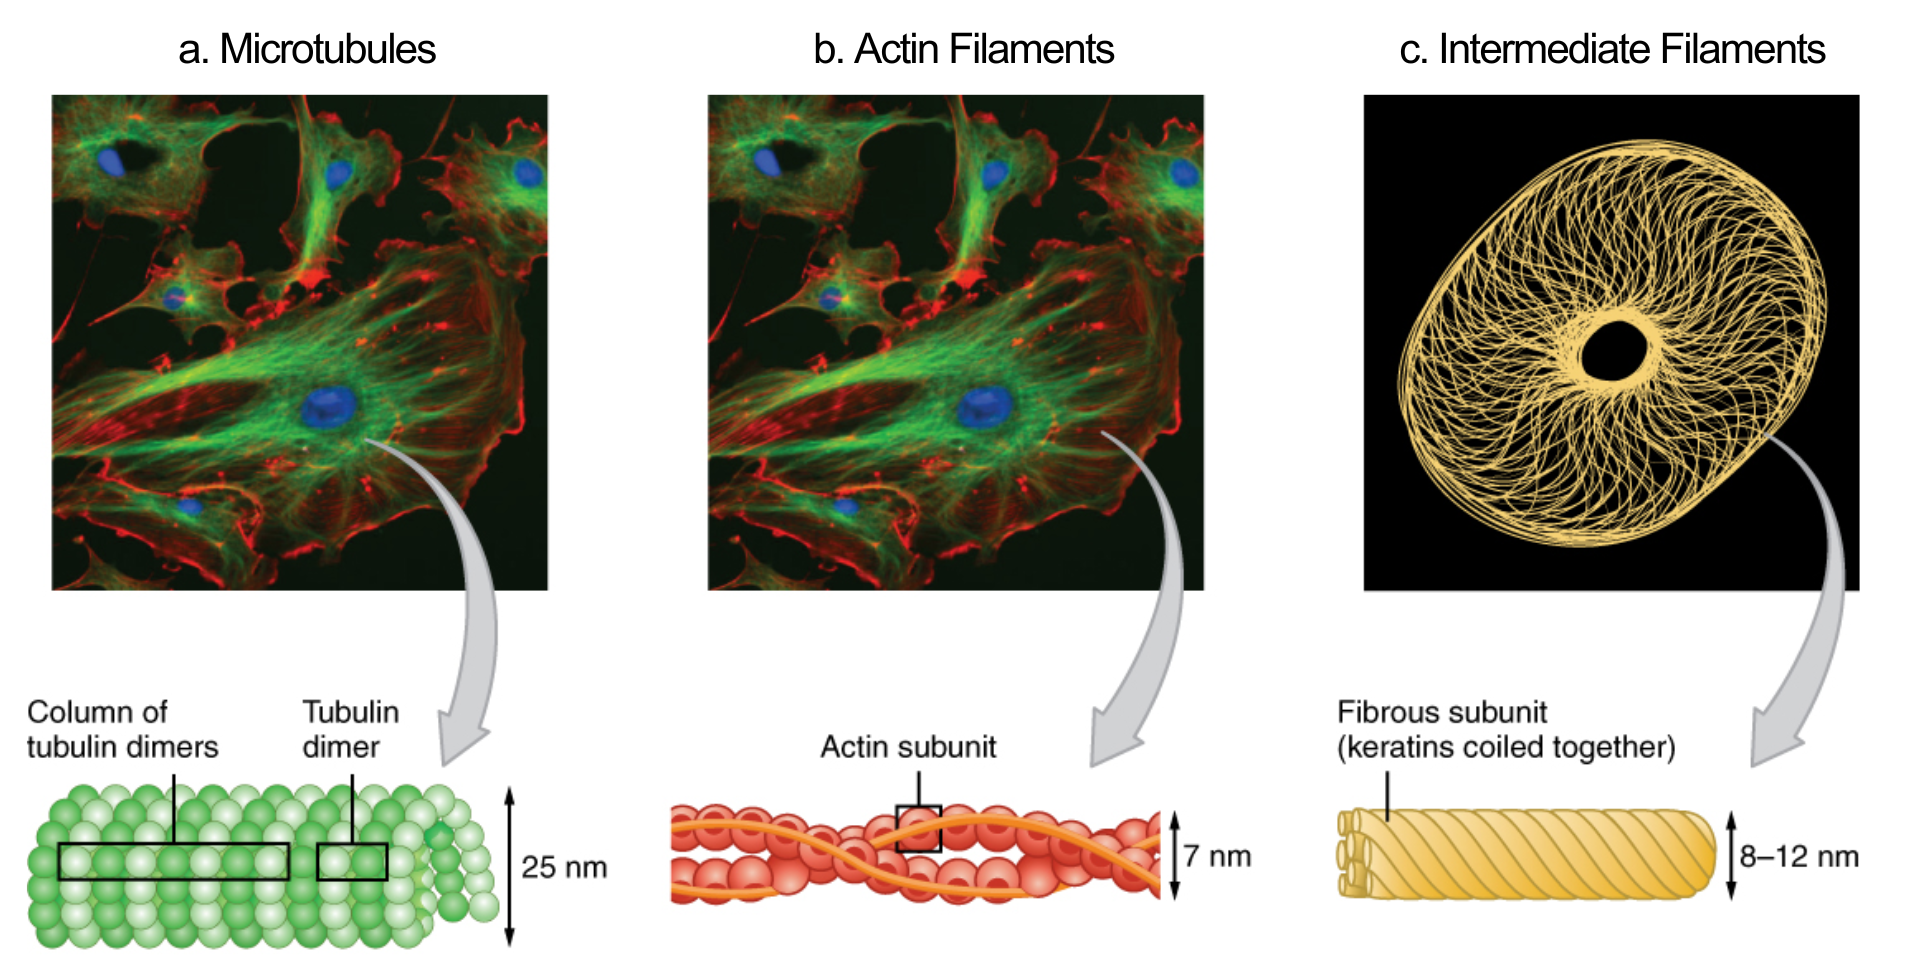
\includegraphics[width=1\textwidth]{figures/section_2/cytoskeleton.png}
    \caption{Structure and components of the cell cytoskeleton. Source: \url{https://shorturl.at/ZCXQS}}\label{fig:cytoskeleton}
\end{figure}

The \textbf{cytoskeleton} is a dynamic network of protein filaments that extend
throughout the cytoplasm of the cell. It is composed of three segments:
\begin{itemize}
    \item \textbf{Microtubules}: Made up of the protein \textbf{tubulin}.
    \item \textbf{Microfilaments}: Made up of the protein \textbf{actin}.
    \item \textbf{Intermediate Filaments}: Made up of \textbf{keratins} coiled together.
\end{itemize}

\begin{figure}[h]
    \centering
    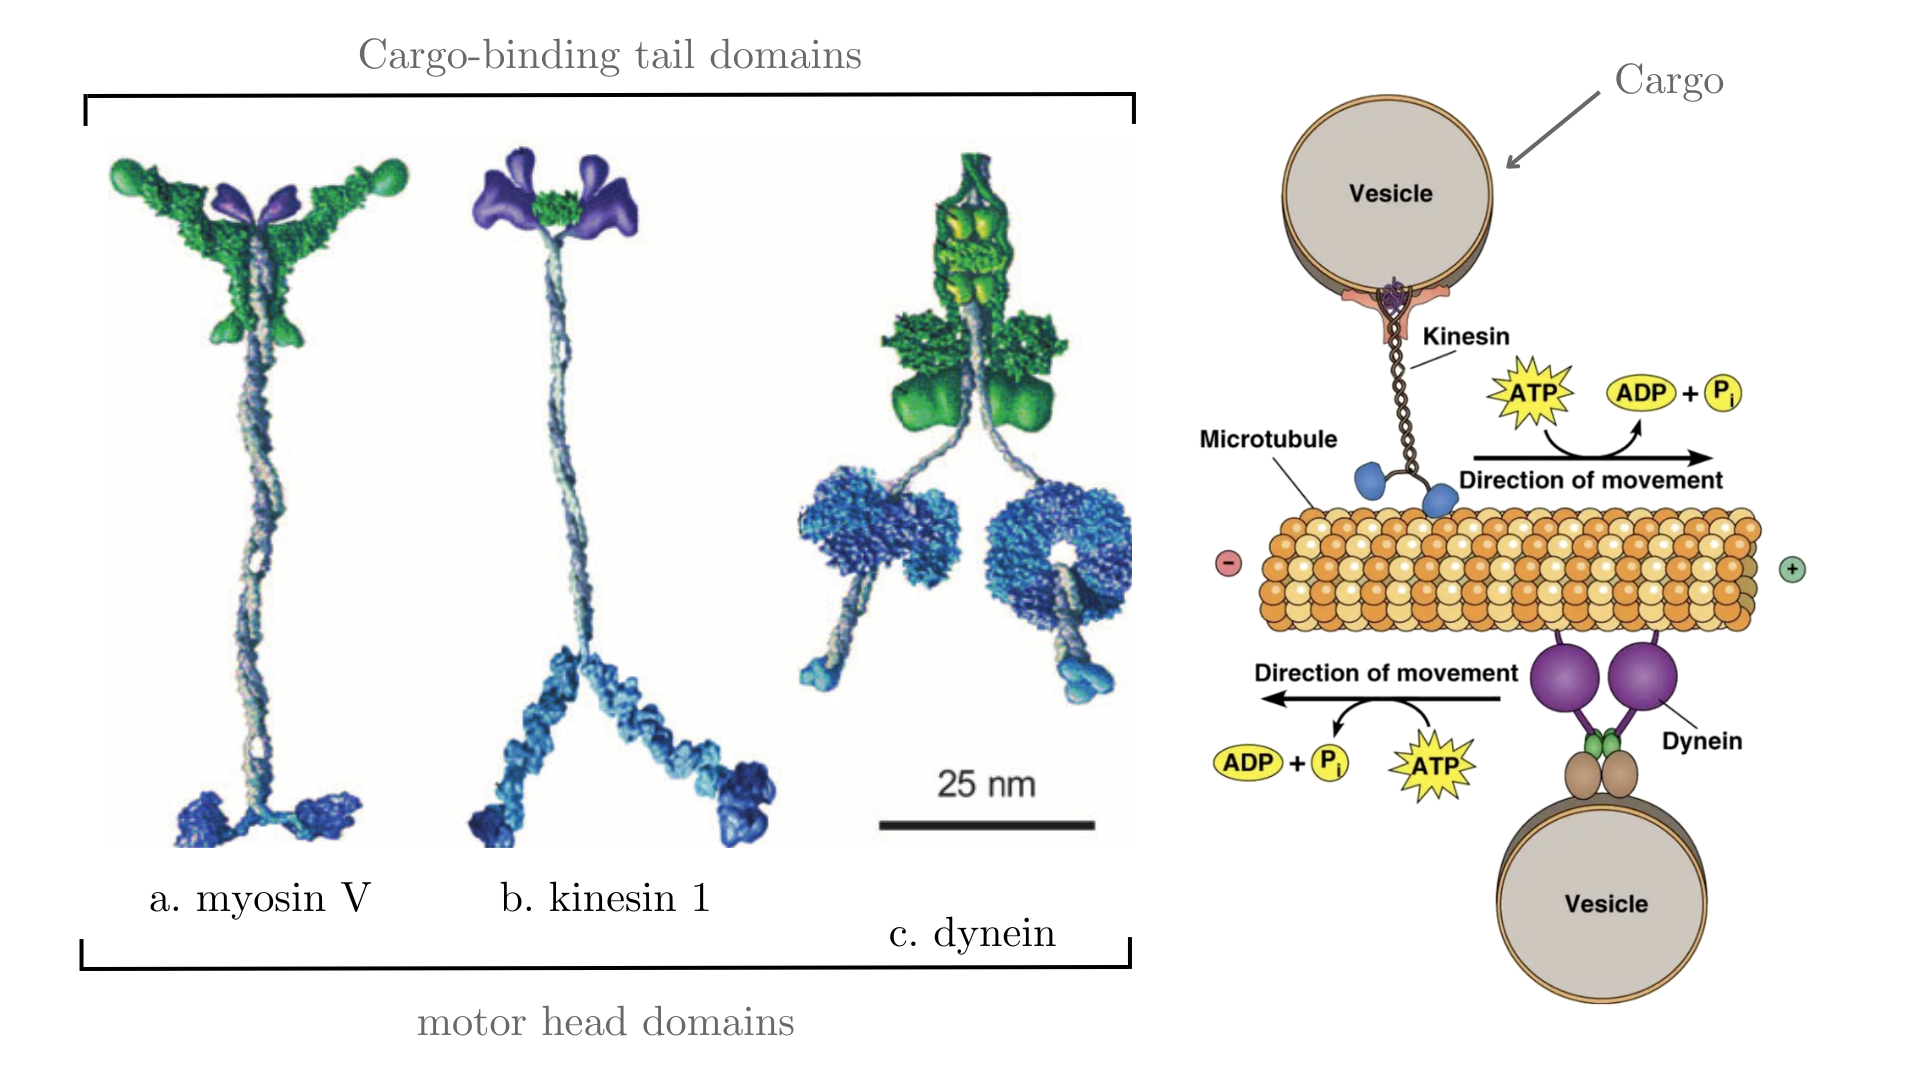
\includegraphics[width=1\textwidth]{figures/section_2/motor_proteins.png}
    \caption{Motor proteins and their movement along cytoskeletal filaments. Modified from \url{https://book.bionumbers.org/how-fast-do-molecular-motors-move-on-cytoskeletal-filaments/}}\label{fig:motor_proteins}
\end{figure}

\textbf{Motor Proteins} are specialized proteins that use energy to move along
cytoskeletal filaments. There are three motor proteins:
\begin{itemize}
    \item \textbf{Myosin V}: Interacts with actin filaments to produce movement.
    \item \textbf{Kinesin}: Transports cargo such as organelles, vesicles, and proteins along microtubules, usually towards the plus (+) end.
    \item \textbf{Dynein}: Moves cargo towards the minus (-) end of microtubules..
\end{itemize}

\subsubsection{Cytoplasm, Organelles, and other Cellular Components}
\textbf{Cytoplasm} is comprised of the cytosol and the cytoskeleton. The cytosolic pH is around 7 and consists of water, dissolved ions, small molecules, and large water-soluble molecules (including proteins\footnote{Not all proteins are water-soluble.}).
\textbf{Organelles} are membrane-bound, lipid bi-layer intracellular compartments. They are suspended in the cytoplasm and are only present in eukaryotic cells. These include smooth / rough Endoplasmic Reticulum, Ribosomes, Mitochondria, Peroxisomes, Lysosomes, Cell Nucleus, and Golgi Apparatus, etc.

\vspace{1em}
\noindent
Role of ER and Golgi Apparatus in protein synthesis:
\begin{itemize}
    \item Rough ER is in the closest proximity to the nucleus. RER consists of ribosomes
          and thus the mRNA it translates are directly secreted into the lumen of the
          RER.
    \item Certain proteins such as membrane proteins, proteins to be trafficked out of
          the cell, and enzymes for lysosomes are secreted out this way whereas other
          proteins are translated via free ribosomes.
    \item Once translated, RER proteins are folded with the help of chaperones and then
          transported to the Golgi apparatus for `Post Translational Modifications (PTM)'
          such as glycosylation, phosphorylation, etc.
\end{itemize}

\noindent
Factors affecting gene expression:
\begin{itemize}
    \item \textbf{Transcription Factors}: Proteins that bind to DNA and regulate the transcription of genes. These are responsible for turning genes on or off and modulating chromatin opening.
    \item \textbf{Spliceosomes}: Spliceosomes are large ribonucleoprotein complexes that are responsible for rearranging exons after splicing. They are found in the nucleus of eukaryotic cells.
    \item \textbf{Epigenetics}: DNA methylation, acetylation, and histone modification are all epigenetic mechanisms that can affect gene expression without altering the underlying DNA sequence.
\end{itemize}

\subsubsection{Extracellular Matrix (ECM)}
\textbf{Extracellular Matrix (ECM)} is a complex network of proteins and carbohydrates secreted by cells into their extracellular environment. This is the non-cellular component in all tissues and organs. It is composed of collagen, proteoglycans, elastin, glycoproteins, and growth factors. ECM provides scaffolding, biochemical and mechanical cues required for tissue homeostasis. Genetic abnormalities in ECM components can lead to severe diseases. It is continuosly remodeled by enzymes such as \textbf{Matrix Metalloproteinases (MMPs)}.
\begin{itemize}
    \item \textbf{Marfan Syndrome}: Caused due to mutation in Fibrillin-1 protein (important for connective tissue integrity). Affects skeleton, heart, eyes, and blood vessels.
    \item \textbf{Ehlers-Danlos Syndrome}: Caused due to mutation in Collagen. Leads to hypermobile joints, stretchy skin, and fragile tissues.
\end{itemize}

\begin{figure}[h!]
    \centering
    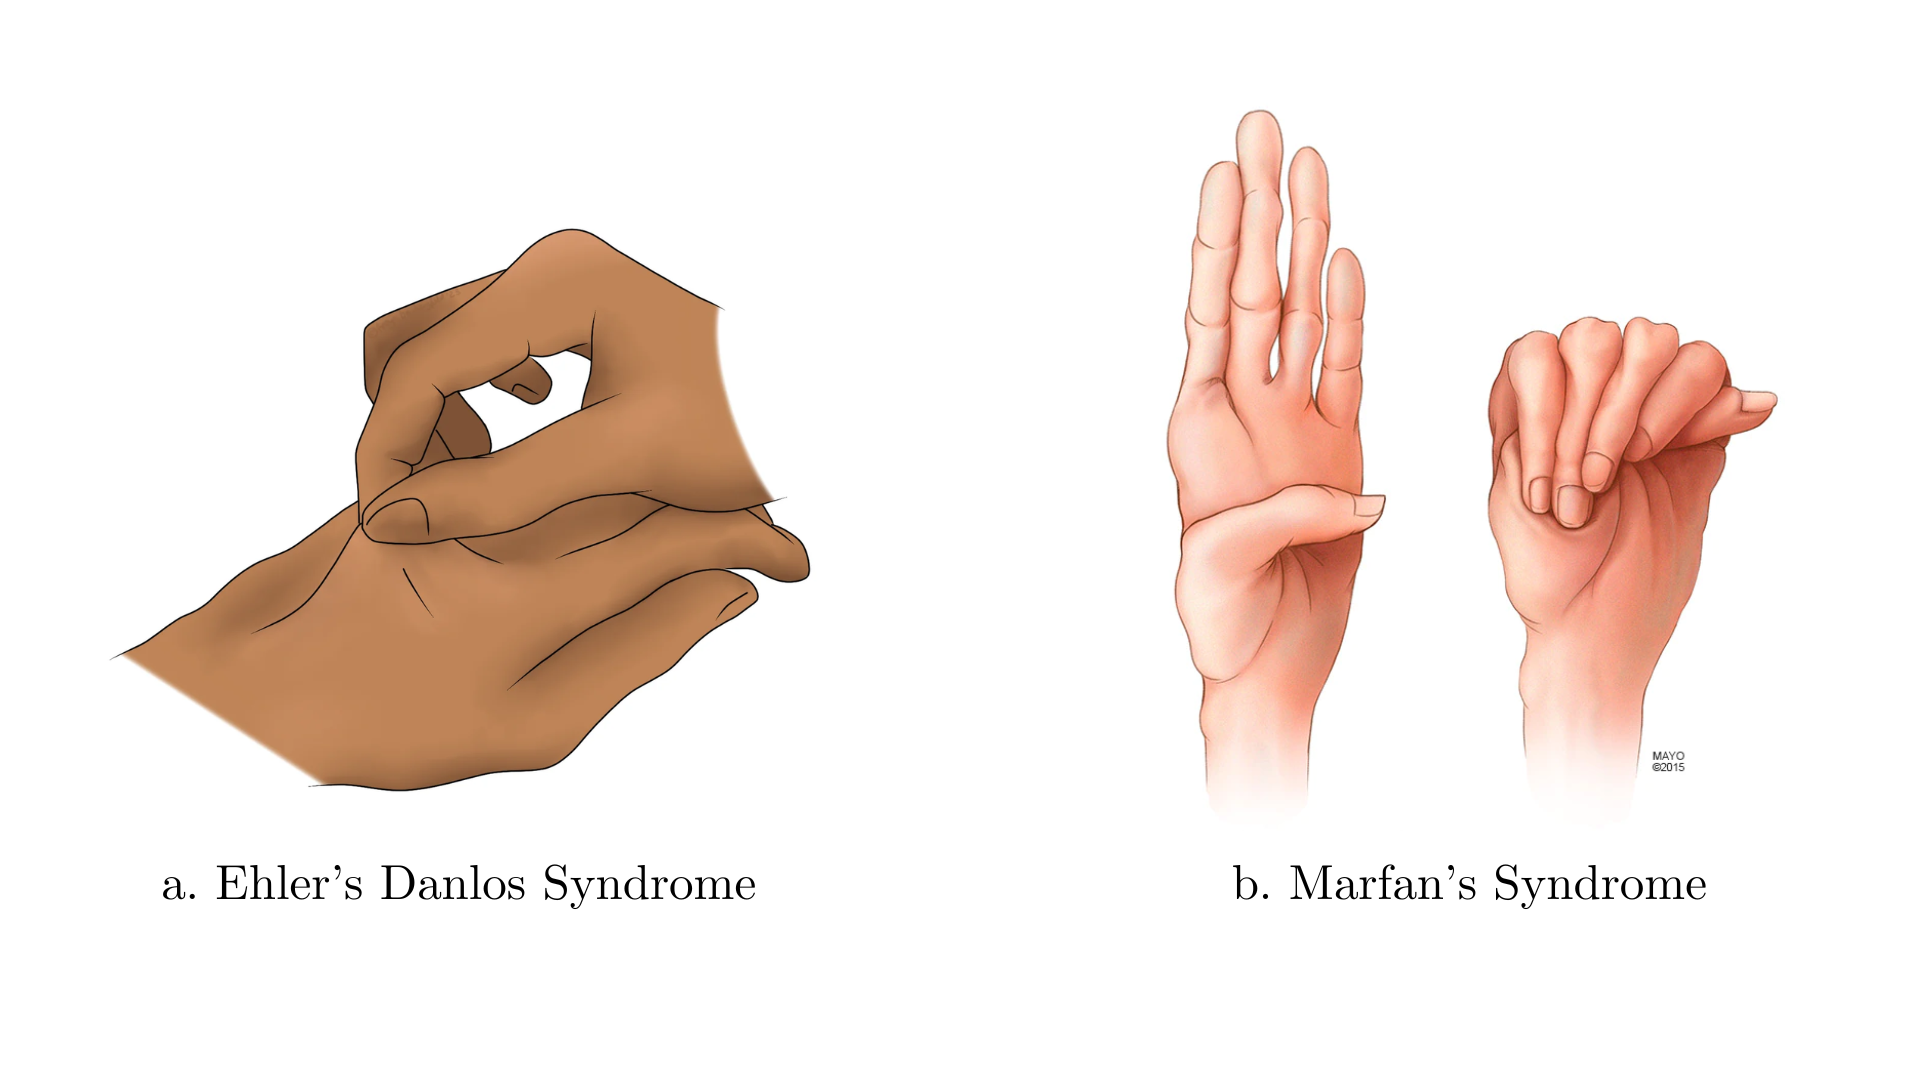
\includegraphics[width=1\textwidth]{figures/section_2/diseases_ecm.png}
    \caption{Diseases caused by ECM abnormalities}\label{fig:diseases_ecm}
\end{figure}

\noindent
Role of Extracellular Matrix (ECM):
\begin{itemize}
    \item \textbf{Anchorage Dependence}: ECM binds to cell surface receptors providing structural stability and positioning.
    \item \textbf{Regulation of Cell Signalling Pathway}: Signalling pathways are initiated when ECM molecules bind to receptors that are essential for gene expression regulation, protein synthesis, etc. Examples incluyde the MAPK pathway.
    \item \textbf{Mechanotransduction}: ECM conveys mechanical signals to cells by alterung shape and tension within the cytoskeleton.
    \item \textbf{Presets Growth Factors}: ECM provides localized and sustained release of growth factors important for tissue repair and growth.
\end{itemize}

\noindent
Various biomaterials that mimic ECM include:
\begin{itemize}
    \item \textbf{Natural ECMs}: Would contain Decellularized ECMs such as Collagen type I fibres,
          Hyaluronic Acid, Fibronectin, etc.
    \item \textbf{Synthetic ECMs}: Peptides, Polymers, and Hydrogels.
\end{itemize}

\subsection{Cell Cultures}
\textbf{Cell lines} are cultures of cells that can be propagated repeatedly and sometimes indefinitely under specified laboratory settings.

Depending on the application, the source of the cell culture can vary. To study
a particular tissue type, cells are derived from that tissue / organ site and
cultured till confluency.
\begin{itemize}
    \item \textbf{Confluency}: The percentage of surface area of a culture dish that is covered by cells.
    \item \textbf{Passaging}: The process of removing cells from a culture dish and adding fresh medium to allow the cells to grow and multiply.
    \item \textbf{Passage Number}: The number of times a cell line has been passaged.
    \item \textbf{Primary and Secondary Cell Lines}: Primary cell lines are cells that are directly taken from an organism's tissues or organs, while secondary cell lines are primary cell lines that have been sub-cultured or passaged.
\end{itemize}

\begin{figure}[h]
    \centering
    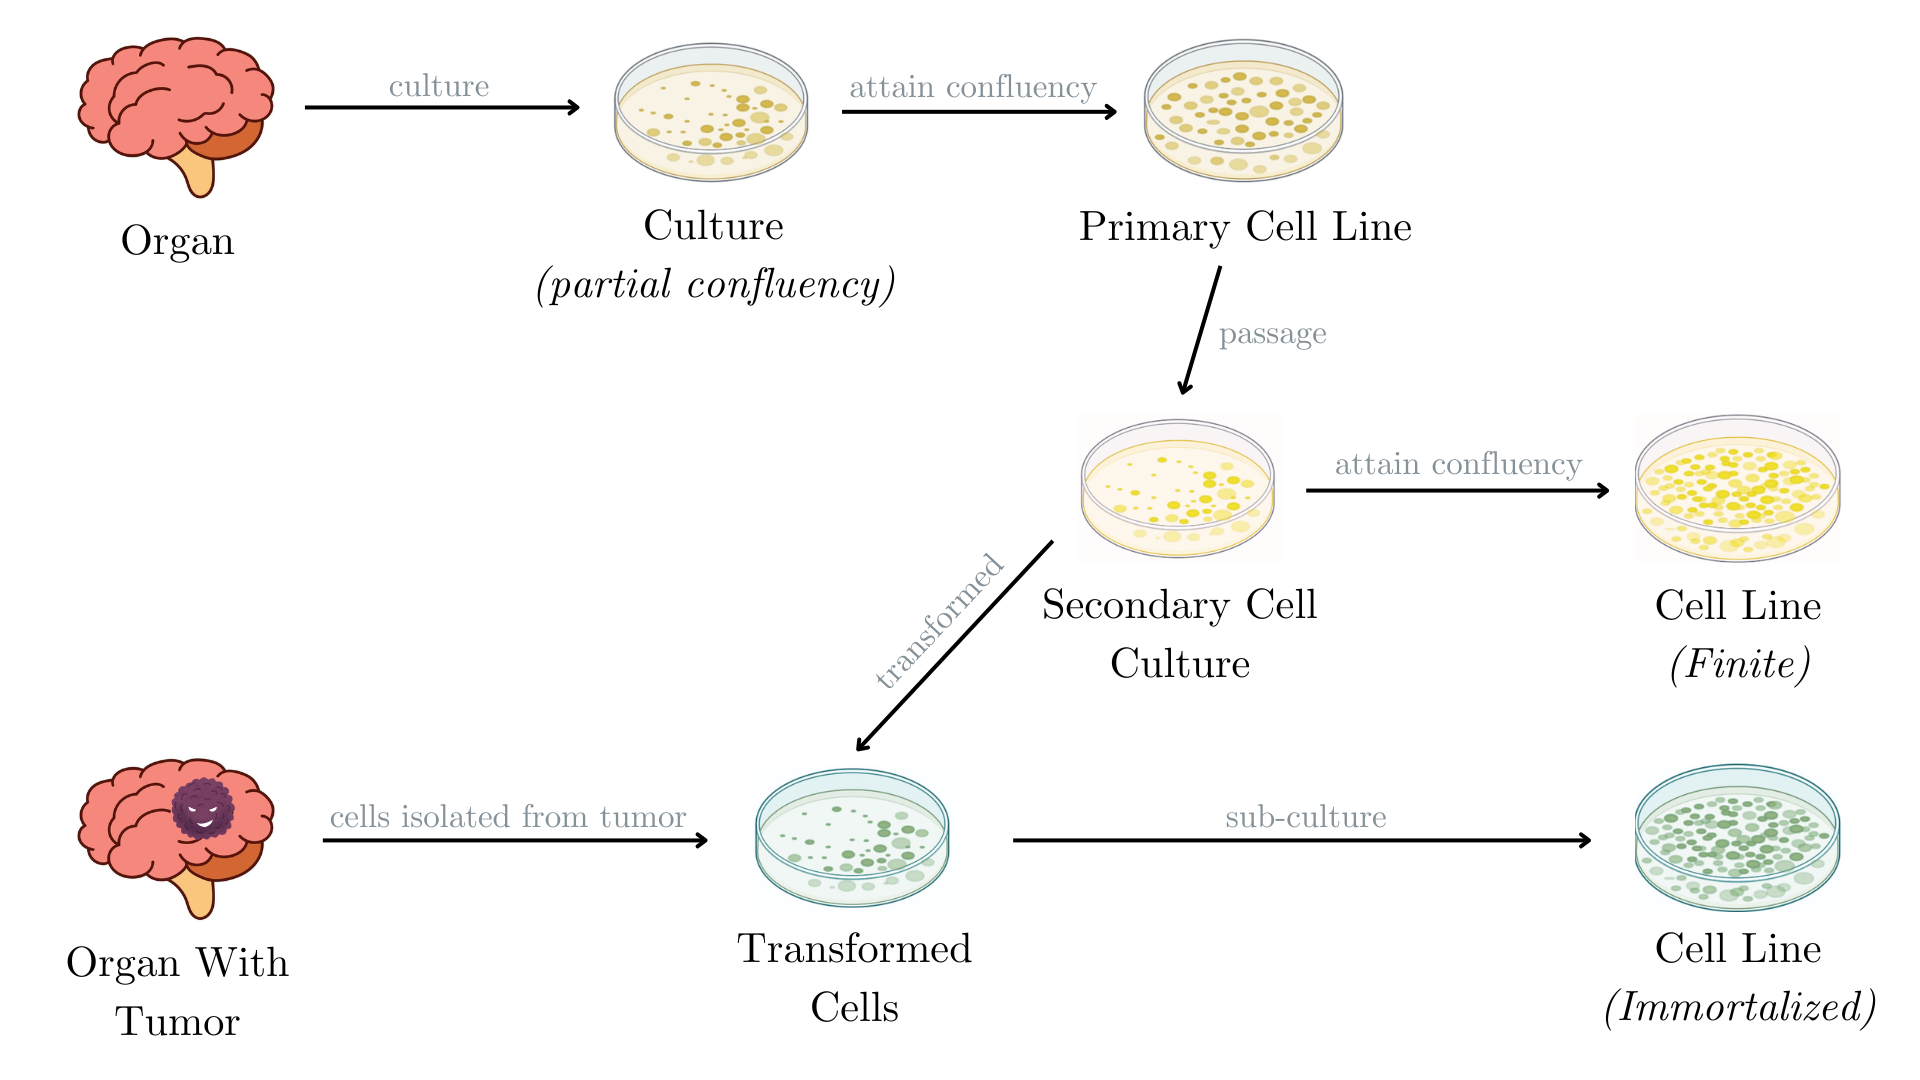
\includegraphics[width=1\textwidth]{figures/section_2/cell_cultures.png}
    \caption{Cell Line Types}\label{fig:cell_line_types}
\end{figure}

Primary cell lines derived from non-stem, non-cancerous sources typically
exhibit a \textbf{finite lifespan} in culture (e.g., skin fibroblasts,
epithelial cells). They undergo a limited number of cell divisions before
entering \textbf{senescence}, a state where they no longer proliferate. This
phenomenon is known as the \textbf{Hayflick Limit}, which is generally around
40--60 passages for human somatic cells.

Once the cells in the primary culture reach confluency, they are passaged and
resuspended in fresh artificial cell culture media. This culture leads to the
formation of a \textbf{secondary cell line}. Usually, these cells might start
loosing phenotype from the primary cell line as they have been present in an
artificial environment for quite some time.

To obtain cell cultures that are immortal, cells are either obtained from a
cancerous source (that have indefinite division capability) or certain
mutations are induced in the non-cancerous cell source to induce indefinite
division capability. This type of cell line is called an \textbf{immortalized
    cell line}.

\section{Metals and Ceramics}
\subsection{Pre-requisites on Interatomic Forces}
Solids are held together by interatomic forces. These forces are of three
types:
\begin{itemize}
    \item \textbf{Ionic Bonds}: Have an electron donor and acceptor. Ionic solids are poor electrical conductors as the $e^{-}$ aren't delocalized and can't travel freely.
    \item \textbf{Covalent Bonds}: Formed between multivalent elements that have equal tendency to share and accept electrons. Also poor electrical conductors. Shared by ceramics and glasses.
    \item \textbf{Metallic Bonds}: Shared by metals. The delocalized $e^{-}$ can move freely within the metal structure, making metals good electrical conductors. The non-localized $e^{-}$ also allows for plastic deformation\footnote{Permanent changes in the shape as opposed to elastic deformation which is reversible changes in shape} making metals ductile.
\end{itemize}

\noindent
Difference between crystalline and amorphous structures:
\begin{itemize}
    \item \textbf{Crystalline} structures have a regular and repeating pattern of atoms (called the unit cell). Present in metals and ceramics.
    \item \textbf{Amorphous} structures have an irregular and non-repeating pattern of atoms. These contain a lot of defects. Eg: Glass.
\end{itemize}

\end{document}
